\documentclass[tikz,border=10pt]{standalone}
\usepackage{amsmath}
\usepackage{tikz}
\usetikzlibrary{arrows.meta, positioning, calc, shapes.geometric}

\begin{document}
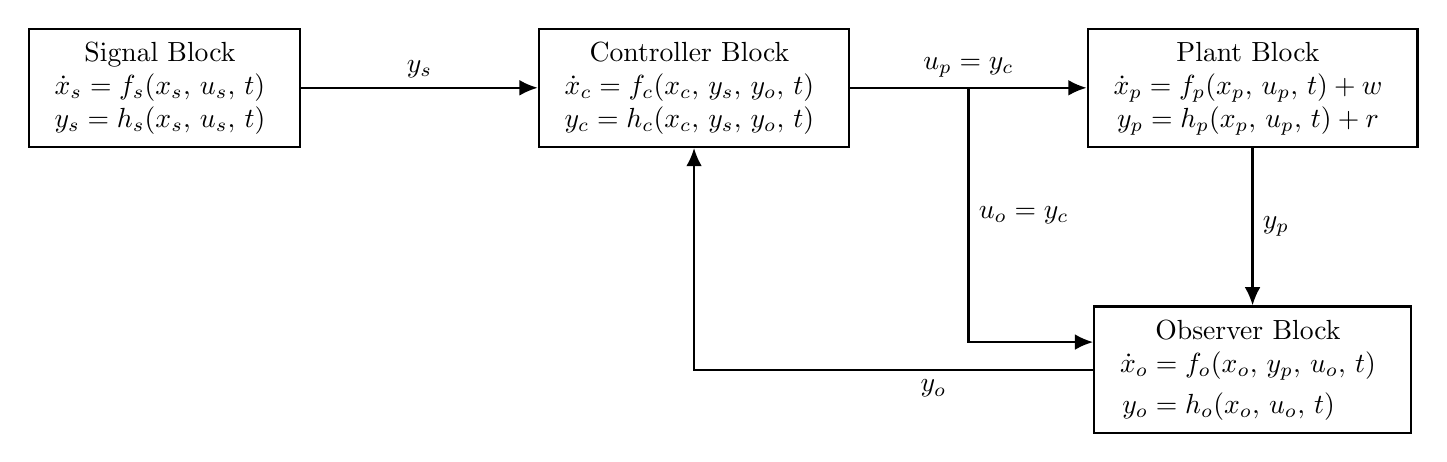
\begin{tikzpicture}[
  block/.style = {draw, thick, minimum height=3em, minimum width=6em, align=center},
  arrow/.style = {thick, -{Latex[width=2mm]}},
  node distance=2.5cm and 2.5cm
]

  % Signal Generator
  \node[block] (siggen) {
    \begin{tabular}{c}
      Signal Block \\
      $\dot{x}_s = f_s(x_s,\, u_s,\, t)$ \\
      $y_s = h_s(x_s,\, u_s,\, t)$
    \end{tabular}
  };

  % Controller (now directly takes r and xhat)
  \node[block, right=3.0cm of siggen] (controller) {
    \begin{tabular}{c}
      Controller Block\\
      $\dot{x}_c = f_c(x_c,\, y_s,\, y_o,\, t)$ \\
      $y_c = h_c(x_c,\, y_s,\, y_o,\, t)$
    \end{tabular}
  };

  % Plant
  \node[block, right=3.0cm of controller] (system) {
    \begin{tabular}{c}
      Plant Block \\
      $\dot{x}_p = f_p(x_p,\, u_p,\, t) + w$ \\
      $y_{p} = h_p(x_p,\, u_p,\, t) + r$
    \end{tabular}
  };

  % Observer
  \node[block, below=2cm of system] (observer) {
    \begin{tabular}{c}
      Observer Block \\
      $\begin{aligned}
        \dot{x}_o &= f_o(x_o,\, y_p,\, u_o,\, t) \\
        y_o       &= h_o(x_o,\, u_o,\, t)
      \end{aligned}$
    \end{tabular}
  };

  % r -> controller
  \draw[arrow] (siggen.east) -- node[above] {$y_s$} (controller.west);

  % controller -> plant
  \draw[arrow] (controller.east) -- node[above] {$u_p = y_c$} (system.west);

  % u branch to observer
  \coordinate (usplit) at ($(controller.east)!0.5!(system.west)$);
  \coordinate[above=1em of observer.west] (observer_uin);
  \draw[arrow] (usplit) |- (observer_uin) node[pos=0.25, right]{$u_o = y_c$};

  % y_p -> observer
  \draw[arrow] (system.south) -- node[right] {$y_p$} (observer.north);

  % observer -> controller (state estimate)
  \coordinate (controller_yoin) at ($(controller.south)!0.5!(controller.south -| observer.north)$);
  \draw[arrow] (observer.west) -| node[pos=0.2, below] {$y_o$} (controller.south);

\end{tikzpicture}
\end{document}
